\chapter{Proximity Preserving Face Redaction}

Face proximity preservation during redaction is crucial for gauging the attention of the subject. We are mainly interested in the relative back-and-forth motion of the face instead of the actual distance of the face from the camera. In the following sections, we describe a method to get the relative proximity of the face from the camera while redacting the face.


%%%%%%%%%%
\section{Proximity using PnP Algorithm}


%%%
\subsection{Methodology}
We employ the PnP (Perspective-n-Point) algorithm to calculate the face proximity from the camera. The algorithm takes 3-D coordinates in an arbitrary world coordinate system as input together with the corresponding 2-D image coordinates and the intrinsic camera parameters, and outputs the extrinsic camera parameters (translation and rotation), i.e., the pose and location of the camera w.r.t. the object defined in an object coordinate system.

We first calibrate the camera using a chessboard pattern and obtain the intrinsic parameters of the camera. Then, we calculate the 3-D facial landmarks (figure \ref{fig:retinaFace3Dlandmarks}) using the Retina Face landmark detector along with redacting the face. Retina Face outputs 68 3-D landmarks in pixel units with the coordinate system centered at the nose-tip. These 3-D coordinates form the 3-D coordinates input to the PnP algorithm. Since Retina Face predicts the 3-D facial landmarks in the pixel coordinate system, the XY of 3-D coordinates forms the corresponding 2-D image coordinates. By using the PnP algorithm, we obtain the proximity of the nose-tip from the camera in pixel units.

\begin{figure}[h]
    \centering
    \captionsetup[subfigure]{justification=centering}
    \subfloat{{
        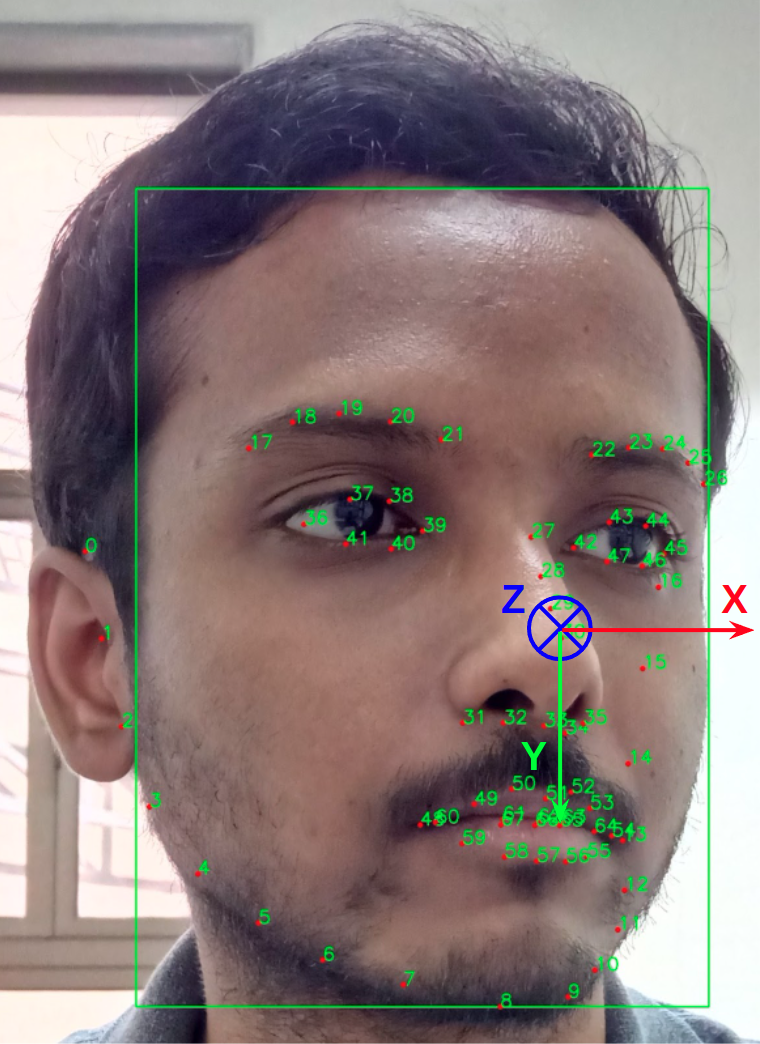
\includegraphics[scale=0.15,valign=m]{DistancePreservingRedaction/RetinaFaceCoordSystem}
        }}
    \quad
    \subfloat{{
        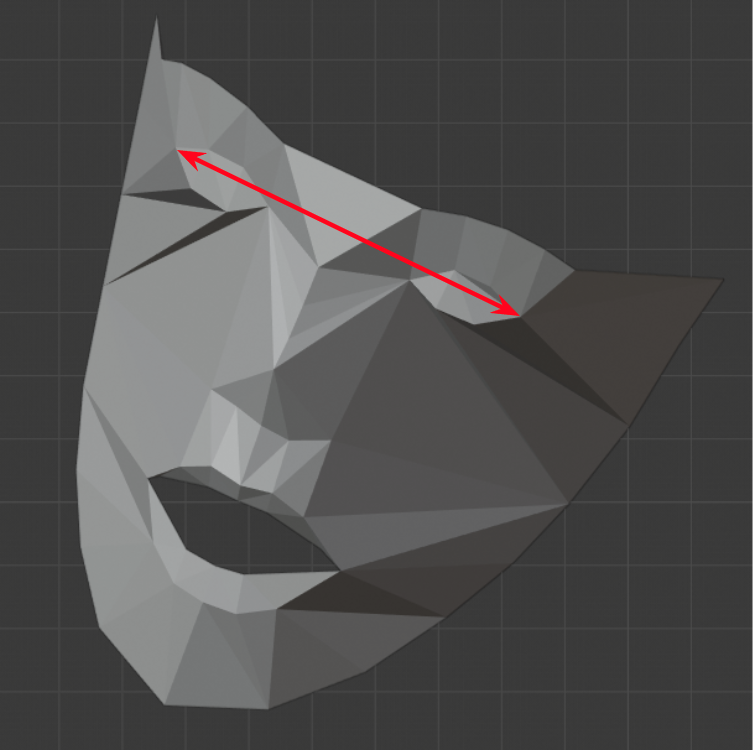
\includegraphics[scale=0.15,valign=m]{DistancePreservingRedaction/EyeExtremitiesDist}
    }}
    \caption{Retina Face: 3-D facial landmarks}
    \label{fig:retinaFace3Dlandmarks}
\end{figure}

Retina Face uses the same coordinate regression method used in Menpo \citep{menpo}, in which a deep neural network is trained jointly for regressing the 2-D and 3-D facial landmark coordinates. This uses a scaled orthographic camera model and scales the world coordinate system to the pixel coordinate system. Thus, the 3-D coordinates output by Retina Face need to be re-scaled back from pixel to world coordinate system. To achieve this, we map the euclidean pixel distance between the two extremes of the eyes (left-most corner of the left eye and right-most corner of the right eye) to the measurements taken in world units in cm. The scale conversion factor thus obtained is used to convert the distance from pixel to cm.


\subsection{Experiments}
To test the above method, we perform experiments in which we record the videos of some subjects gradually going away from the camera and subsequently coming closer to the camera. We then calculate the face proximity of each frame in the video and plot the proximity versus time curve.

\begin{figure}[h]
    \centering
    \captionsetup[subfigure]{justification=centering}
    \subfloat{{
        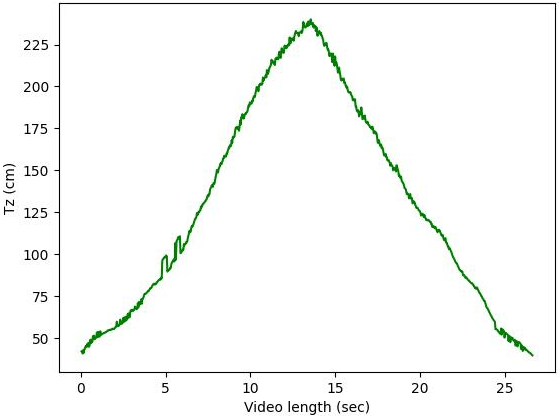
\includegraphics[scale=0.35]{DistancePreservingRedaction/plot-1}
        }}
    \quad
    \subfloat{{
        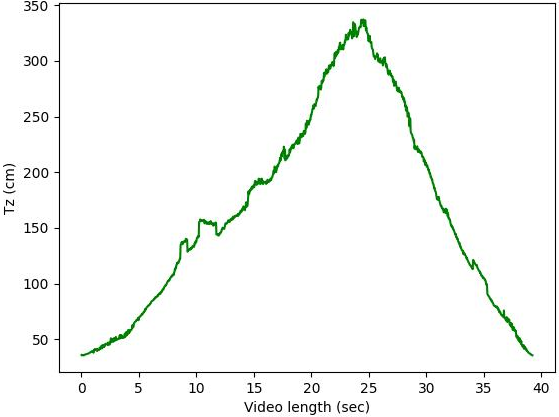
\includegraphics[scale=0.35]{DistancePreservingRedaction/plot-2}
    }}
    \quad
    \subfloat{{
        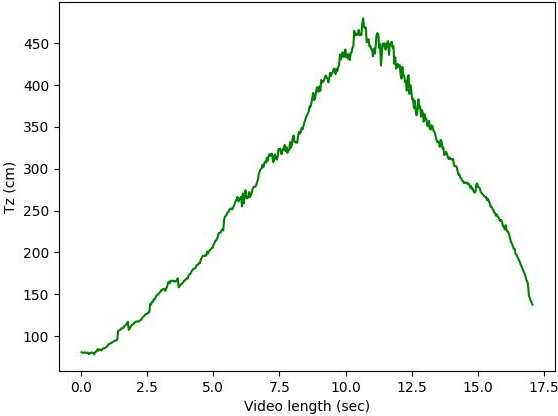
\includegraphics[scale=0.35]{DistancePreservingRedaction/plot-3}
    }}
    \quad
    \subfloat{{
        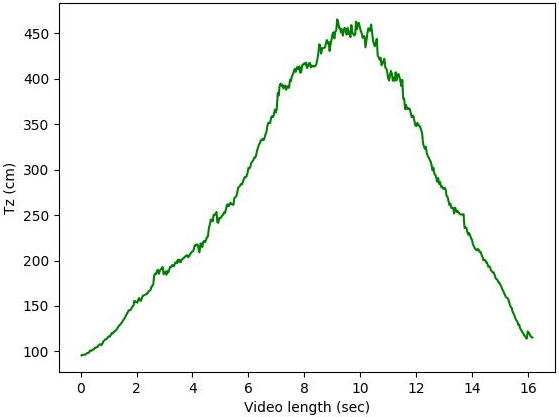
\includegraphics[scale=0.35]{DistancePreservingRedaction/plot-4}
    }}
    \caption[Proximity v/s Time curves]{Examples of Proximity v/s Time of video Curves}
    \label{fig:distCurve}
\end{figure}

\begin{figure}[h]
  \centering
    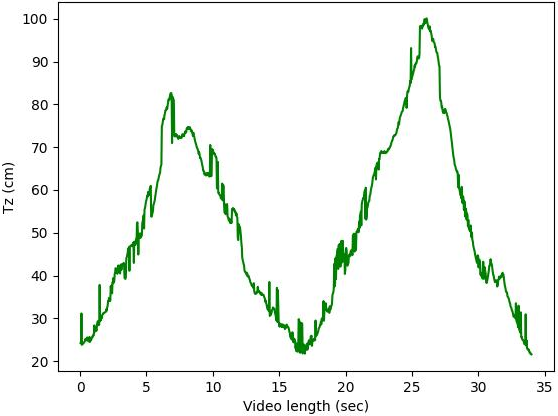
\includegraphics[scale=0.35]{DistancePreservingRedaction/plot-6}
    \caption[Proximity v/s Time curve in-the-wild]{Proximity v/s Time of video Curve for in-the-wild video}
    \label{fig:distCurve_inTheWild} 
\end{figure}

The curves in figure \ref{fig:distCurve} show some examples of facial proximity versus time plots we obtained for some of the videos. The videos on which we calculate these plots can be found \href{https://drive.google.com/drive/folders/1HEZISJiaaP0LAooNuELbls8TPWqtTL0M?usp=sharing}{here}.

We also simulated the in-the-wild nature of the 2-way START dataset where the subjects are relatively closer to the camera and the facial proximity fluctuates back and forth much more rapidly, along with large variations in the pose. In this video, the subject moves back and forth twice with large variations in pose, and as expected, there are two peaks in the proximity versus time curve shown in figure \ref{fig:distCurve_inTheWild}.

We also calculated the face proximity values for some images with measured ground truth values (the images along with their ground truths can be found \href{https://drive.google.com/drive/folders/1MsDul6SAmFN9JhgleApR6tdFm79J5AoK?usp=sharing}{here}). Table \ref{tab:proximityOnGrTrImages} shows the ground truth and the values predicted by our algorithm.

\begin{table}[h]
  \centering
    \caption{Face Proximity on Images with Ground Truths}
    \label{tab:proximityOnGrTrImages}
    \begin{tabular}{ | >{\centering\arraybackslash} m{2cm} || >{\centering\arraybackslash} m{1cm} | >{\centering\arraybackslash} m{1cm} | >{\centering\arraybackslash} m{1cm} | >{\centering\arraybackslash} m{1cm} | >{\centering\arraybackslash} m{1cm} | >{\centering\arraybackslash} m{1cm} | >{\centering\arraybackslash} m{1cm} |
    >{\centering\arraybackslash} m{1cm} |} 
        \hline
        \textbf{Ground Truth (cm)} & 54.3 & 71.5 & 101 & 126 & 177.6 & 224.1 & 271.1 & 321.5\\
        \hline
        \textbf{Prediction (cm)} & 65.9 & 85.7 & 121.7 & 149.9 & 211.6 & 261.1 & 320.1 & 381.1\\
        \hline
    \end{tabular}
\end{table}